\documentclass[12pt,a4paper]{article}

% -------------------- Пакеты --------------------
\usepackage{fontspec}
\usepackage{polyglossia}
\setmainlanguage{russian}
\setotherlanguage{english}
\IfFontExistsTF{Times New Roman}{\setmainfont{Times New Roman}}{\setmainfont{Liberation Serif}}
\IfFontExistsTF{Times New Roman}{\newfontfamily\cyrillicfont{Times New Roman}}{\newfontfamily\cyrillicfont{Liberation Serif}}

\usepackage[a4paper, left=20mm, right=20mm, top=20mm, bottom=20mm]{geometry}
\usepackage{amsmath, amssymb}
\usepackage{graphicx}
\usepackage{float}
\usepackage{booktabs}
\usepackage{array}
\usepackage{longtable}
\usepackage{tabularx}
\usepackage{multirow}
\usepackage{indentfirst}
\usepackage{titlesec}
\usepackage{caption}
\usepackage{subcaption}
\usepackage{hyperref}
\usepackage{xcolor}
\usepackage{listings}
\usepackage{microtype}

\hypersetup{
    colorlinks=true,
    linkcolor=black,
    urlcolor=blue,
    citecolor=black
}

\graphicspath{{figure_4.03/}}
\setlength{\parindent}{1.25cm}
\setlength{\parskip}{0.2em}
\titleformat{\section}{\normalfont\Large\bfseries}{\thesection}{1em}{}
\titleformat{\subsection}{\normalfont\large\bfseries}{\thesubsection}{1em}{}

\captionsetup{labelsep=period}

\newcommand{\um}{\ensuremath{\,\mu\text{м}}}
\newcommand{\nm}{\ensuremath{\,\text{нм}}}
\newcommand{\cm}{\ensuremath{\,\text{см}}}

\begin{document}

\begin{titlepage}
\begin{center}
Санкт-Петербургский национальный исследовательский институт\\
информационных технологий, механики и оптики

\vspace{3cm}

{\Large\bfseries ОТЧЁТ ПО ЛАБОРАТОРНОЙ РАБОТЕ №4.03}

\vspace{0.5cm}

{\large\bfseries «Определение радиуса кривизны линзы\\
по интерференционной картине колец Ньютона»}

\vspace{2.5cm}
\end{center}

\begin{flushleft}
Группа: Z3244

Студенты:\\
Поминов Вадим\\
Забродский Александр\\
Фадеев Марк

Преподаватель:\\
Калантаевский Иван Эдуардович
\end{flushleft}

\vfill

\begin{flushleft}
К работе допущен:\\[0.4cm]
Работа выполнена:\\[0.4cm]
Отчет принят:
\end{flushleft}

\end{titlepage}

\section{Цель работы}

Изучение интерференционной картины колец Ньютона.

\section{Задачи}

\begin{enumerate}
    \item Определение радиуса кривизны плоско-выпуклой линзы с помощью интерференционной картины колец Ньютона.
    \item Оценка спектральной полосы пропускания оптических фильтров.
\end{enumerate}

\section{Объект исследования}

Объектом исследования является интерференционная картина колец Ньютона, возникающая в воздушном зазоре между плоско-выпуклой линзой и плоскопараллельной стеклянной пластиной.

\section{Метод исследования}

В работе используется метод наблюдения интерференции в отраженном свете. Радиусы темных колец Ньютона определяются по измеренным диаметрам колец. Далее строится зависимость $r^2(n)$, где $r$ -- радиус темного кольца, а $n$ -- его номер. Радиус кривизны линзы определяется по разности квадратов радиусов двух темных колец. Дополнительно по положению исчезновения видности интерференционной картины оценивается ширина полосы пропускания светофильтра.

\section{Рабочие формулы и исходные данные}

Для воздушного зазора между линзой и пластиной показатель преломления принимаем равным $n \approx 1$. Тогда для темных колец Ньютона выполняется связь
\begin{equation}
    r_m^2 = m\lambda R,
\end{equation}
где $r_m$ -- радиус темного кольца порядка $m$, $\lambda$ -- длина волны света, $R$ -- радиус кривизны линзы.

Так как из-за пыли, малой деформации стекла и неидеального контакта центральная область может давать систематическое смещение, радиус кривизны удобнее находить по разности квадратов радиусов двух колец:
\begin{equation}
    R = \frac{r_m^2-r_n^2}{(m-n)\lambda}.
\end{equation}

Радиус кольца находится по измеренному диаметру:
\begin{equation}
    r = \frac{d}{2}.
\end{equation}

Для проверки линейности зависимости $r^2(n)$ используется аппроксимация методом наименьших квадратов:
\begin{equation}
    r^2 = k n + b.
\end{equation}
Если зависимость близка к линейной, то по угловому коэффициенту можно оценить радиус кривизны:
\begin{equation}
    R_{\text{МНК}} = \frac{k}{\lambda}.
\end{equation}

Для оценки спектральной ширины полосы пропускания фильтра используется формула
\begin{equation}
    \Delta \lambda = \frac{2\lambda^2 R}{2r_{\text{dis}}^2 + R\lambda},
\end{equation}
где $r_{\text{dis}}$ -- расстояние от центра интерференционной картины до точки исчезновения видности.

Частотная ширина полосы пропускания связана с шириной по длинам волн выражением
\begin{equation}
    \Delta \nu = \frac{c\Delta\lambda}{\lambda^2}.
\end{equation}

В работе использовались следующие длины волн:
\begin{equation}
    \lambda_{blue}=435.8\nm,\quad
    \lambda_{green}=546.1\nm,\quad
    \lambda_{orange}=578.4\nm,\quad
    \lambda_{red}=630\nm.
\end{equation}

Все основные расчеты радиуса кривизны выполнялись в системе СГС: радиусы колец переводились в сантиметры, длины волн -- в сантиметры. При этом $1\um = 10^{-4}\cm$, $1\nm = 10^{-7}\cm$.

\section{Измерительные приборы}

\begin{table}[H]
\centering
\caption{Измерительные приборы и элементы установки}
\begin{tabularx}{\textwidth}{>{\raggedright\arraybackslash}X>{\raggedright\arraybackslash}X>{\raggedright\arraybackslash}X}
\toprule
Наименование & Назначение & Особенности использования \\
\midrule
Микроскоп с камерой & Получение изображения колец Ньютона & Фокусировка на интерференционной картине \\
Программа Altami Studio & Измерение диаметров колец & Измерение проводилось по изображению с камеры \\
Набор светофильтров & Выделение заданной длины волны & Использовались синий, зеленый, оранжевый и красный фильтры \\
Плоско-выпуклая линза и стеклянная пластина & Получение воздушного зазора переменной толщины & Формирование интерференционной картины колец Ньютона \\
Источник света & Освещение системы линза--пластина & Яркость подбиралась так, чтобы кольца были видны достаточно четко \\
\bottomrule
\end{tabularx}
\end{table}

\section{Проведение измерений}

Система линза--пластина устанавливалась на столике микроскопа. После установки соответствующего светофильтра проводилась настройка микроскопа и источника света до получения четкой картины колец Ньютона. Для каждого фильтра измерялись диаметры четырех темных колец. Каждое измерение диаметра проводилось три раза.

После измерения диаметров вычислялись радиусы колец. Затем для каждого фильтра было определено расстояние от центра картины до точки, где видность интерференционной картины становится нулевой. При повторных измерениях радиуса исчезновения видности получились совпадающие значения. Это означает, что статистический разброс по серии измерений формально равен нулю. Однако реальная погрешность измерения не равна нулю, так как точка исчезновения контраста определяется визуально по изображению. Поэтому для дальнейших расчетов принимаем погрешность определения радиуса нулевой видности
\begin{equation}
    \Delta r_{\text{dis}} = 25\um.
\end{equation}

\section{Результаты прямых измерений и их обработка}

В таблицах ниже приведены радиусы колец, рассчитанные как половины измеренных диаметров. Значение $\overline r$ является средним по трем измерениям.

\subsection{Зеленый светофильтр, $\lambda = 546.1\nm$}

\begin{table}[H]
\centering
\small
\caption{Радиусы темных колец для зеленого светофильтра}
\begin{tabular}{cccccc}
\toprule
$n$ & $r_1$, мкм & $r_2$, мкм & $r_3$, мкм & $\overline r$, мкм & $\overline r^2$, см$^2$ \\
\midrule
1 & 1178.624 & 1179.269 & 1146.071 & 1167.988 & 0.01364 \\
2 & 1457.895 & 1452.477 & 1453.371 & 1454.581 & 0.02116 \\
3 & 1656.866 & 1662.566 & 1670.332 & 1663.255 & 0.02766 \\
4 & 1875.034 & 1879.778 & 1867.673 & 1874.161 & 0.03512 \\
\bottomrule
\end{tabular}
\end{table}

\subsection{Красный светофильтр, $\lambda = 630\nm$}

\begin{table}[H]
\centering
\small
\caption{Радиусы темных колец для красного светофильтра}
\begin{tabular}{cccccc}
\toprule
$n$ & $r_1$, мкм & $r_2$, мкм & $r_3$, мкм & $\overline r$, мкм & $\overline r^2$, см$^2$ \\
\midrule
1 & 1235.866 & 1254.742 & 1231.712 & 1240.773 & 0.01540 \\
2 & 1543.884 & 1525.849 & 1538.745 & 1536.159 & 0.02360 \\
3 & 1789.888 & 1772.277 & 1789.531 & 1783.899 & 0.03182 \\
4 & 1996.737 & 2001.499 & 2021.011 & 2006.416 & 0.04026 \\
\bottomrule
\end{tabular}
\end{table}

\subsection{Оранжевый светофильтр, $\lambda = 578.4\nm$}

\begin{table}[H]
\centering
\small
\caption{Радиусы темных колец для оранжевого светофильтра}
\begin{tabular}{cccccc}
\toprule
$n$ & $r_1$, мкм & $r_2$, мкм & $r_3$, мкм & $\overline r$, мкм & $\overline r^2$, см$^2$ \\
\midrule
1 & 1208.052 & 1223.341 & 1195.386 & 1208.926 & 0.01462 \\
2 & 1521.420 & 1495.061 & 1487.822 & 1501.434 & 0.02254 \\
3 & 1740.783 & 1730.134 & 1724.079 & 1731.665 & 0.02999 \\
4 & 1918.874 & 1939.237 & 1923.678 & 1927.263 & 0.03714 \\
\bottomrule
\end{tabular}
\end{table}

\subsection{Синий светофильтр, $\lambda = 435.8\nm$}

\begin{table}[H]
\centering
\small
\caption{Радиусы темных колец для синего светофильтра}
\begin{tabular}{cccccc}
\toprule
$n$ & $r_1$, мкм & $r_2$, мкм & $r_3$, мкм & $\overline r$, мкм & $\overline r^2$, см$^2$ \\
\midrule
1 & 1144.857 & 1142.851 & 1145.001 & 1144.236 & 0.01309 \\
2 & 1388.306 & 1392.101 & 1393.293 & 1391.233 & 0.01936 \\
3 & 1598.725 & 1590.886 & 1606.945 & 1598.852 & 0.02556 \\
4 & 1786.779 & 1780.027 & 1777.368 & 1781.391 & 0.03173 \\
\bottomrule
\end{tabular}
\end{table}

\section{Построение графиков $r^2(n)$}

По средним значениям радиусов для каждого фильтра построены зависимости $r^2(n)$. Точки на графиках соответствуют экспериментальным данным, прямая -- МНК-аппроксимации.

\begin{figure}[H]
    \centering
    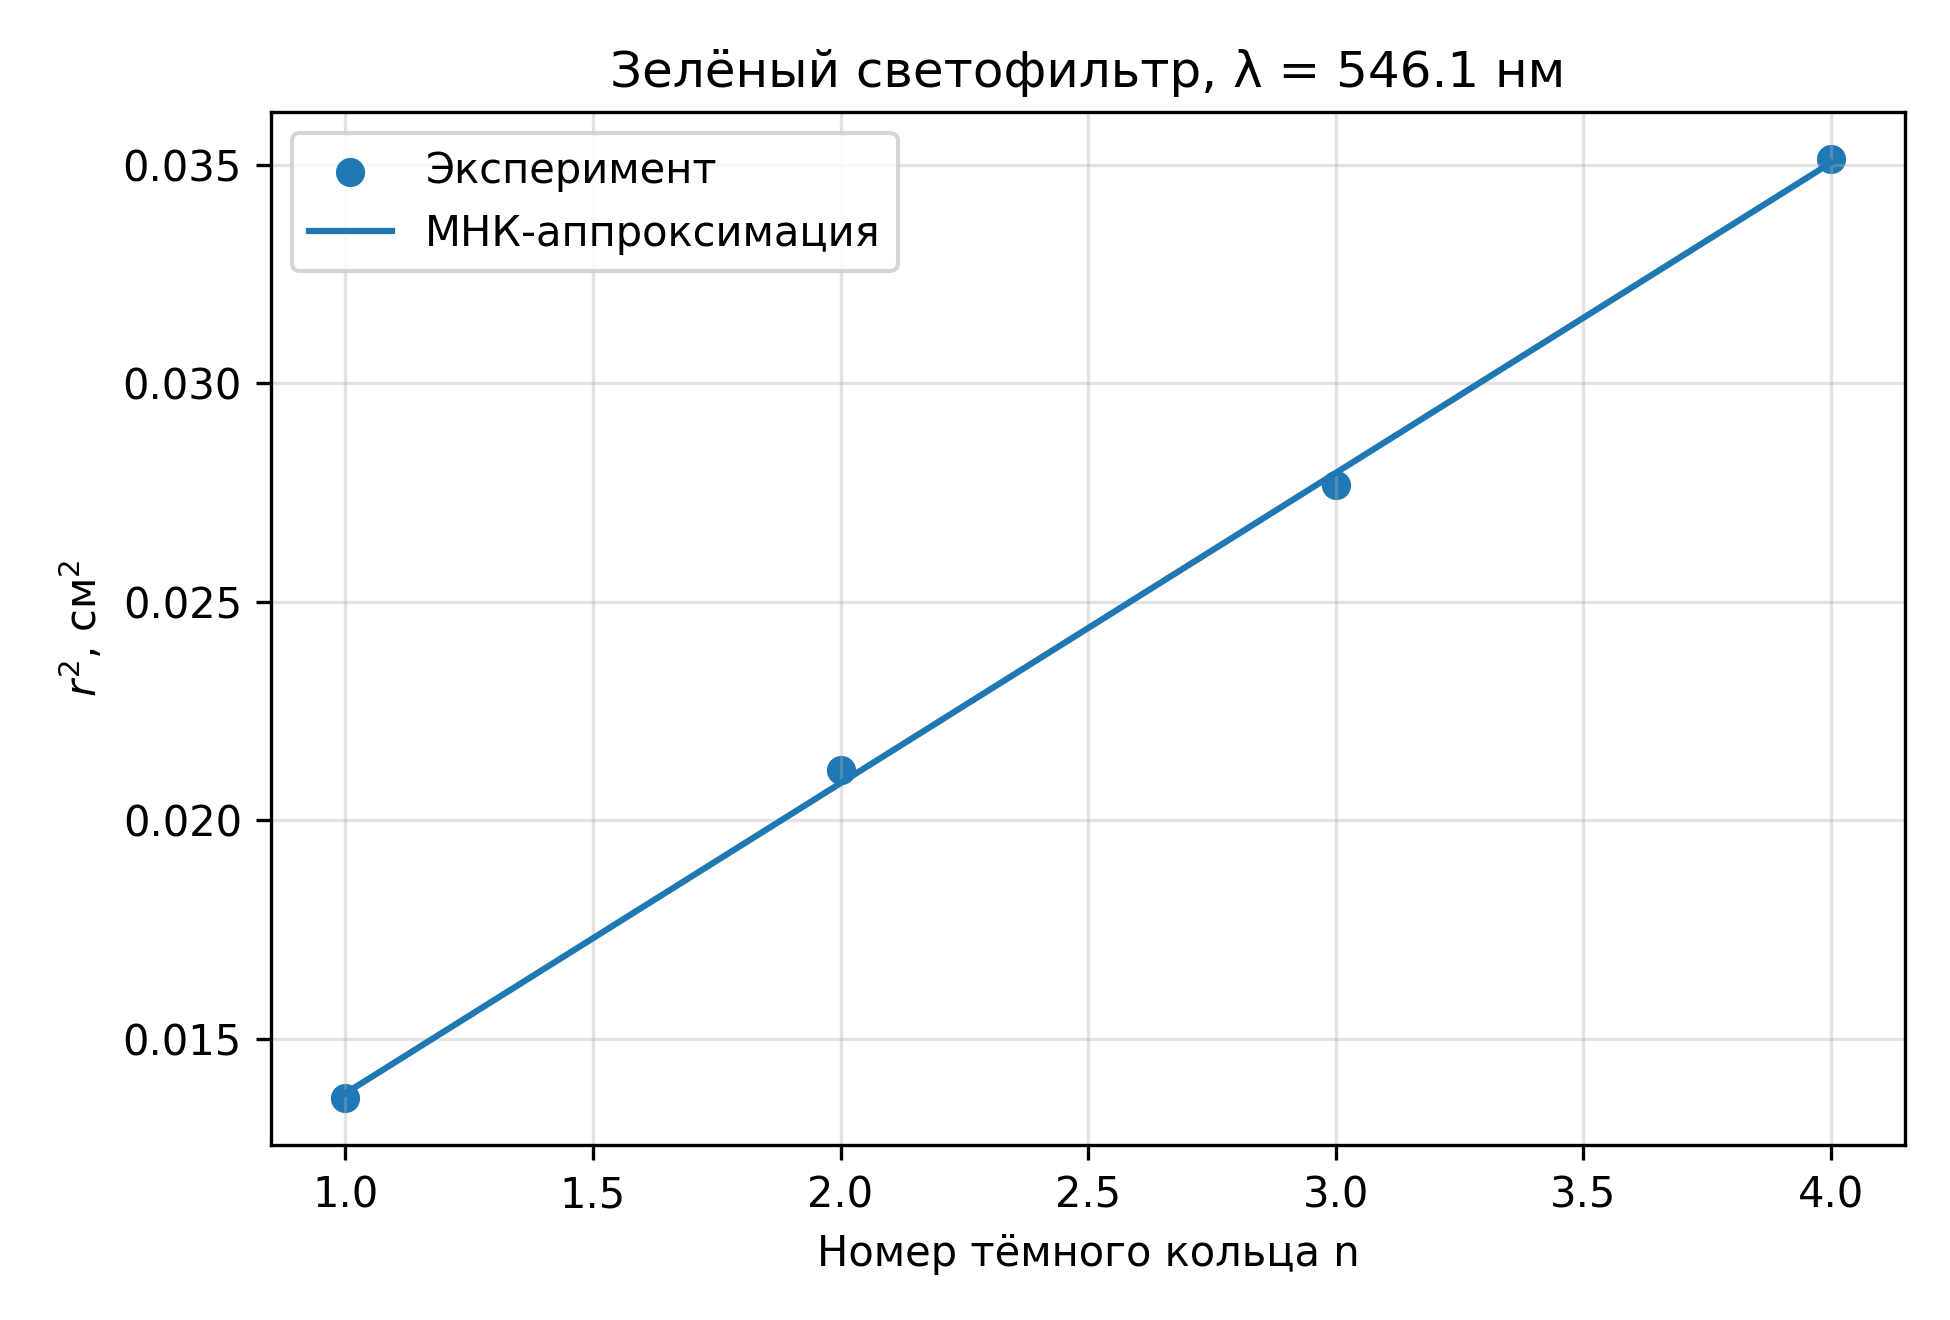
\includegraphics[width=0.82\textwidth]{r2_green.png}
    \caption{Зависимость $r^2(n)$ для зеленого светофильтра.}
\end{figure}

\begin{figure}[H]
    \centering
    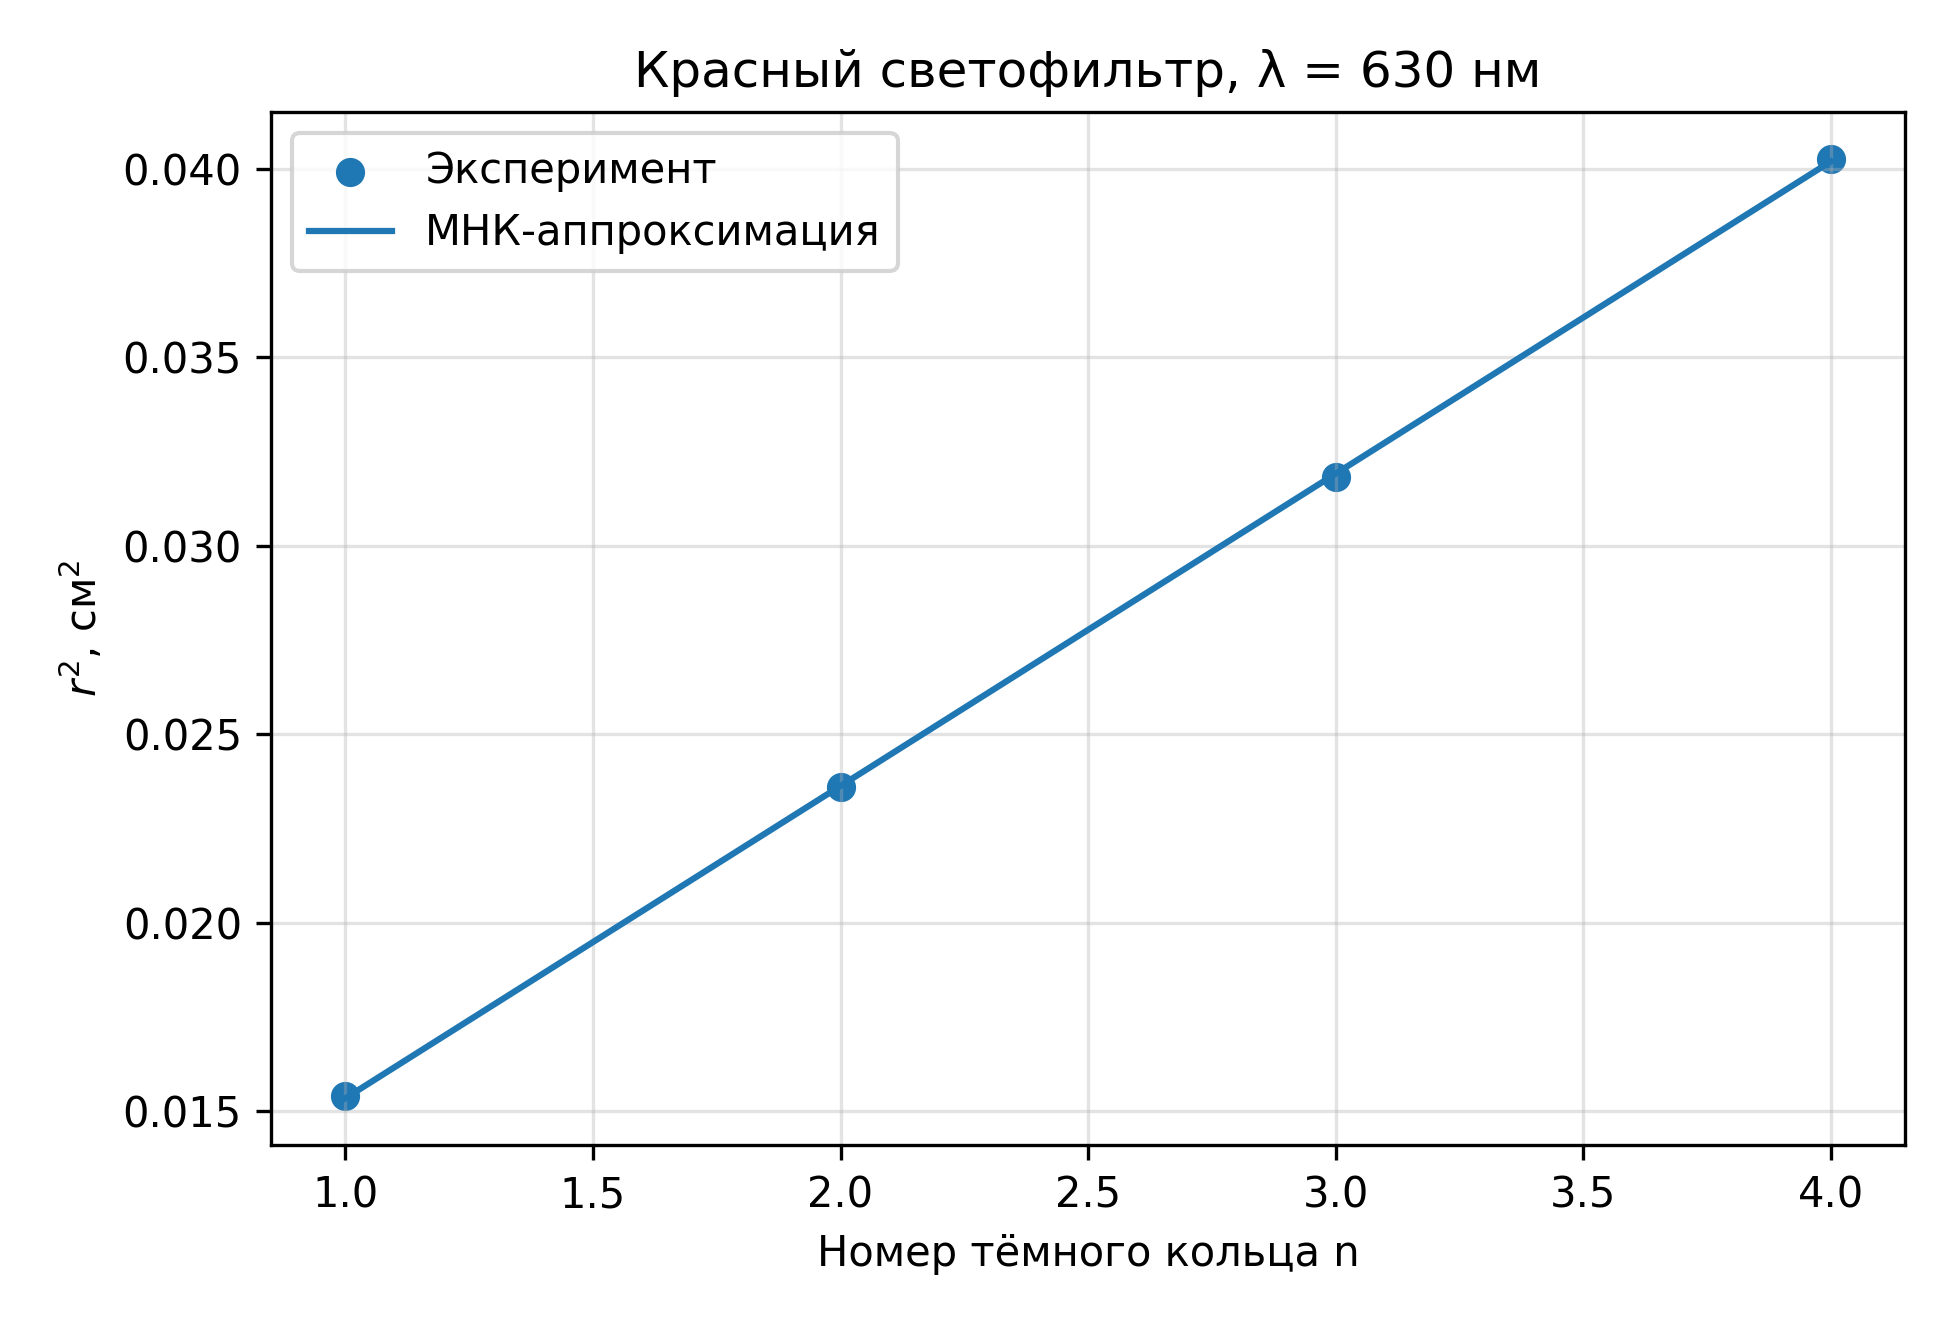
\includegraphics[width=0.82\textwidth]{r2_red.png}
    \caption{Зависимость $r^2(n)$ для красного светофильтра.}
\end{figure}

\begin{figure}[H]
    \centering
    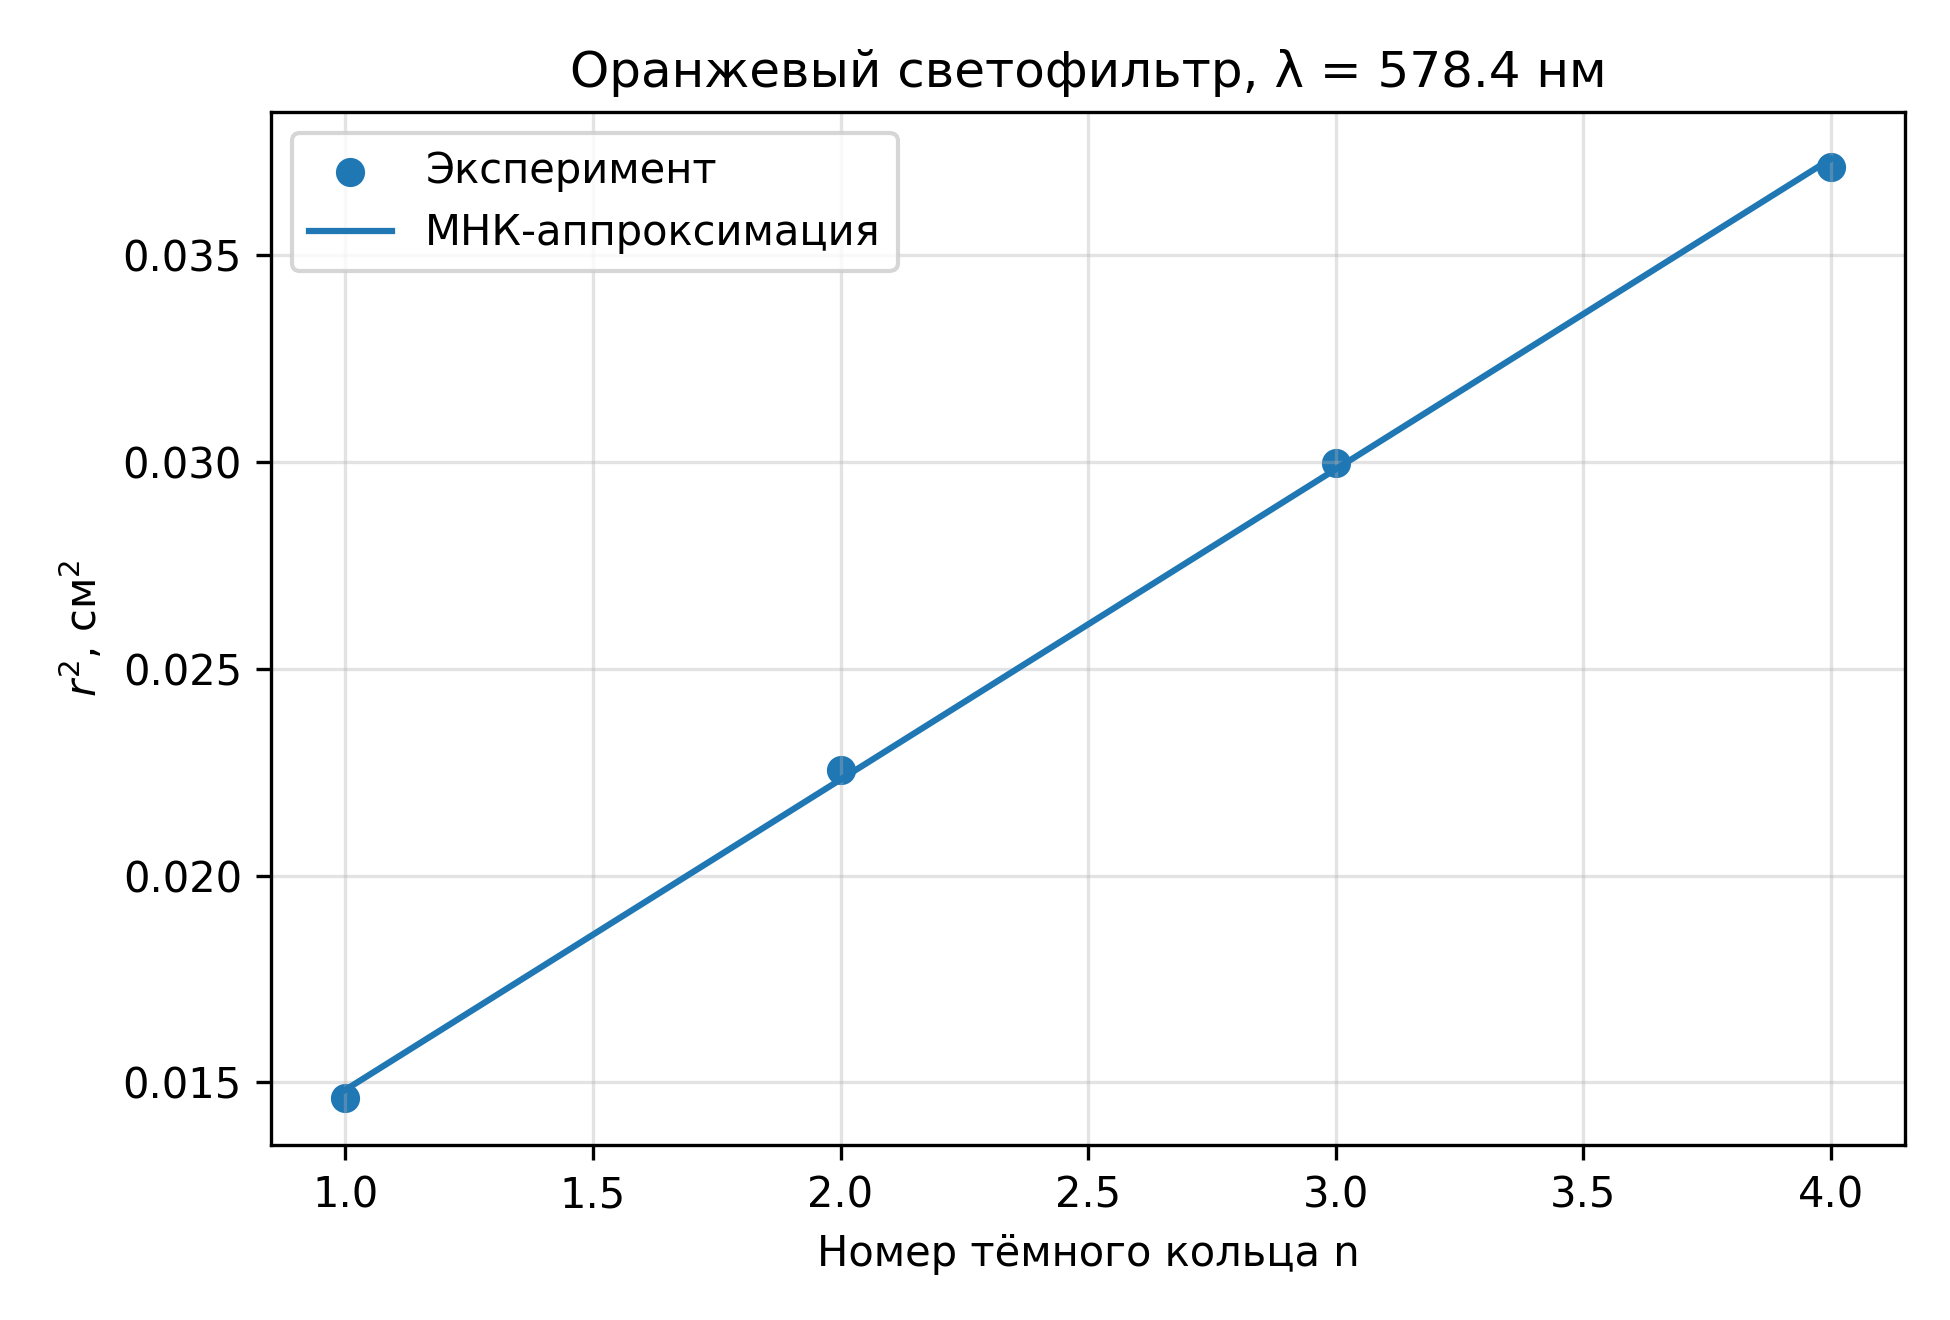
\includegraphics[width=0.82\textwidth]{r2_orange.png}
    \caption{Зависимость $r^2(n)$ для оранжевого светофильтра.}
\end{figure}

\begin{figure}[H]
    \centering
    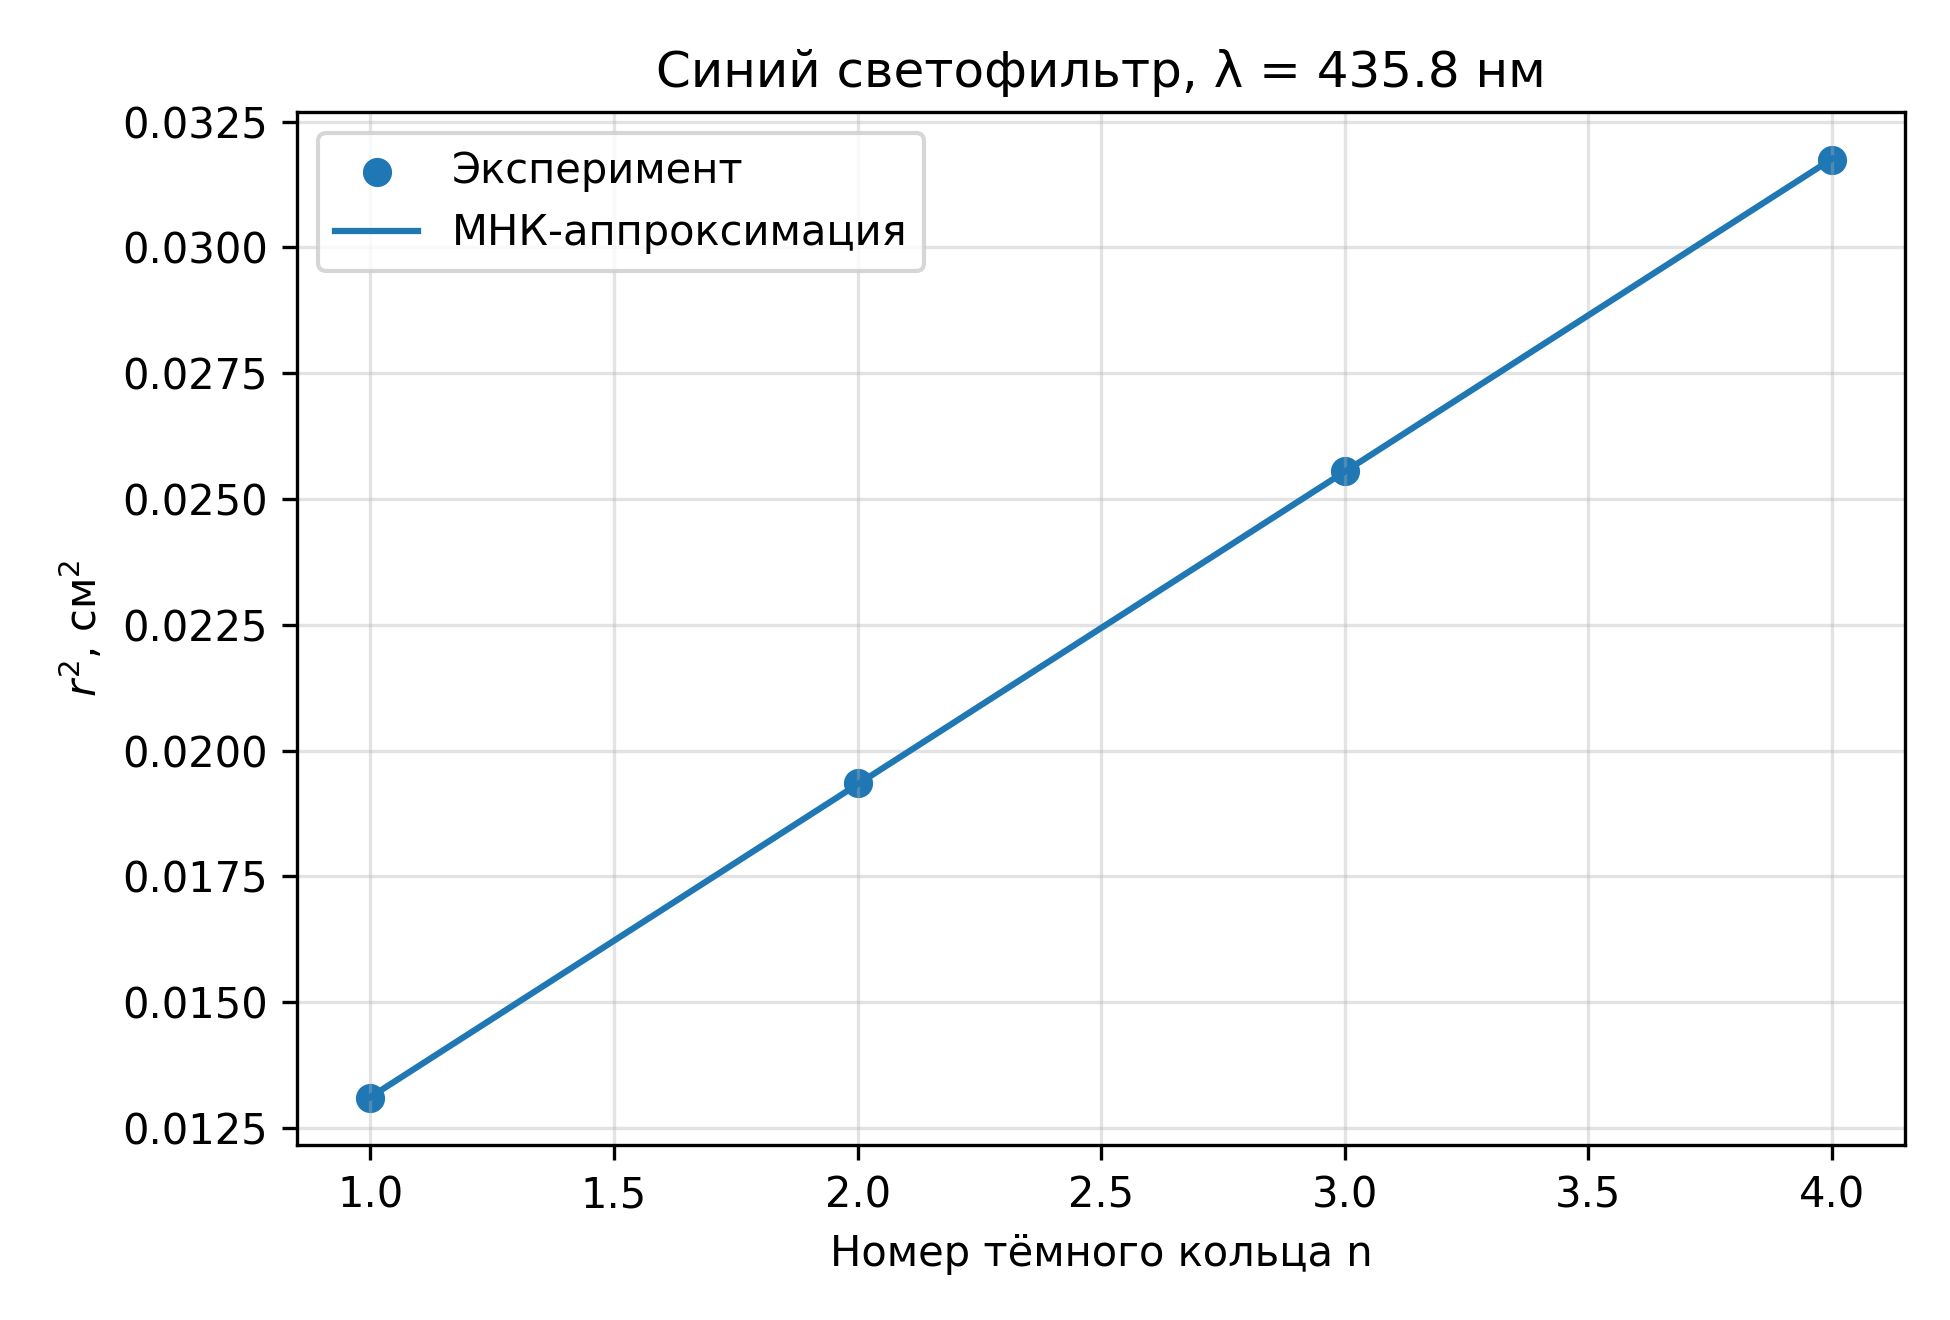
\includegraphics[width=0.82\textwidth]{r2_blue.png}
    \caption{Зависимость $r^2(n)$ для синего светофильтра.}
\end{figure}

Полученные зависимости близки к линейным, что согласуется с формулой $r_m^2 = m\lambda R$ для темных колец Ньютона.

\section{Расчет радиуса кривизны линзы}

Для каждого фильтра радиус кривизны был рассчитан по двум парам колец: $(4,2)$ и $(3,1)$. Дополнительно в таблице приведена оценка $R_{\text{МНК}}$, полученная из углового коэффициента прямой $r^2(n)$.

\begin{table}[H]
\centering
\small
\caption{Расчет радиуса кривизны линзы}
\begin{tabular}{lccccc}
\toprule
Светофильтр & $\lambda$, нм & $R_{\text{МНК}}$, см & $R_{4,2}$, см & $R_{3,1}$, см & $\overline R$, см \\
\midrule
Зеленый & 546.1 & 129.9 & 127.9 & 128.4 & 128.1 \\
Красный & 630.0 & 131.4 & 132.2 & 130.4 & 131.3 \\
Оранжевый & 578.4 & 129.7 & 126.2 & 132.9 & 129.5 \\
Синий & 435.8 & 142.6 & 142.0 & 143.1 & 142.5 \\
\bottomrule
\end{tabular}
\end{table}

Покажем пример расчета для зеленого светофильтра по паре колец $(4,2)$:
\begin{equation}
    R_{4,2}=\frac{r_4^2-r_2^2}{(4-2)\lambda}
    =\frac{0.0351248-0.0211581}{2\cdot 546.1\cdot 10^{-7}}
    \approx 127.9\cm.
\end{equation}

Аналогично были рассчитаны остальные значения. Среднее значение по восьми рассчитанным значениям радиуса:
\begin{equation}
    \overline R = 132.9\cm.
\end{equation}

\section{Оценка полосы пропускания фильтров}

Результаты измерения радиуса исчезновения видности приведены в таблице. Для синего фильтра, как и для остальных фильтров, использовались три одинаковых повторных значения.

\begin{table}[H]
\centering
\small
\caption{Радиус исчезновения видности интерференционной картины}
\begin{tabular}{lccccc}
\toprule
Светофильтр & $\lambda$, нм & $r_1$, мкм & $r_2$, мкм & $r_3$, мкм & $\overline r_{\text{dis}}$, мкм \\
\midrule
Зеленый & 546.1 & 5038.732 & 5038.732 & 5038.732 & 5038.732 \\
Красный & 630.0 & 5571.593 & 5571.593 & 5571.593 & 5571.593 \\
Оранжевый & 578.4 & 4579.429 & 4579.429 & 4579.429 & 4579.429 \\
Синий & 435.8 & 6798.092 & 6798.092 & 6798.092 & 6798.092 \\
\bottomrule
\end{tabular}
\end{table}

Для расчета использовалось итоговое значение радиуса кривизны линзы $R=132.9\cm$. Например, для зеленого фильтра:
\begin{equation}
    \Delta\lambda =
    \frac{2\lambda^2 R}{2r_{\text{dis}}^2+R\lambda}
    =\frac{2\cdot(546.1\cdot10^{-7})^2\cdot132.9}{2\cdot(5038.732\cdot10^{-4})^2+132.9\cdot546.1\cdot10^{-7}}
    \approx 15.4\nm.
\end{equation}

Итоговые значения полосы пропускания фильтров приведены в таблице.

\begin{table}[H]
\centering
\small
\caption{Оценка спектральной полосы пропускания фильтров}
\begin{tabular}{lcccc}
\toprule
Светофильтр & $\lambda$, нм & $r_{\text{dis}}$, мкм & $\Delta\lambda$, нм & $\Delta\nu$, ТГц \\
\midrule
Зеленый & 546.1 & 5038.732 & $15.4 \pm 0.6$ & $15.5 \pm 0.6$ \\
Красный & 630.0 & 5571.593 & $16.8 \pm 0.7$ & $12.7 \pm 0.5$ \\
Оранжевый & 578.4 & 4579.429 & $20.8 \pm 0.8$ & $18.7 \pm 0.8$ \\
Синий & 435.8 & 6798.092 & $5.4 \pm 0.2$ & $8.6 \pm 0.3$ \\
\bottomrule
\end{tabular}
\end{table}

\section{Расчет погрешностей}

Для оценки погрешности радиуса кривизны использовались восемь значений $R$, полученных по двум парам колец для четырех светофильтров. Среднее значение:
\begin{equation}
    \overline R = \frac{1}{N}\sum_{i=1}^{N} R_i, \quad N=8.
\end{equation}

Среднеквадратичное отклонение:
\begin{equation}
    s_R = \sqrt{\frac{\sum\limits_{i=1}^{N}(R_i-\overline R)^2}{N-1}}.
\end{equation}

Доверительный интервал для вероятности $P=0.95$ оценивался по формуле
\begin{equation}
    \Delta R = t_{0.95;7}\frac{s_R}{\sqrt{N}}.
\end{equation}

По расчетам:
\begin{equation}
    s_R = 6.4\cm, \quad t_{0.95;7}=2.365,
\end{equation}
\begin{equation}
    \Delta R = 2.365\cdot\frac{6.4}{\sqrt{8}}\approx 5.3\cm.
\end{equation}

Следовательно,
\begin{equation}
    R = (132.9 \pm 5.3)\cm.
\end{equation}

Для ширины полосы пропускания была использована формула распространения погрешностей:
\begin{equation}
    \Delta(\Delta\lambda)=
    \sqrt{\left(\frac{\partial f}{\partial R}\Delta R\right)^2+
    \left(\frac{\partial f}{\partial r}\Delta r\right)^2},
\end{equation}
где
\begin{equation}
    f(R,r)=\frac{2\lambda^2R}{2r^2+R\lambda}.
\end{equation}

Погрешность $\Delta r_{\text{dis}}$ была принята равной $25\um$, поскольку точка исчезновения контраста определялась визуально по изображению.

\section{Окончательные результаты}

\begin{enumerate}
    \item Радиус кривизны исследуемой плоско-выпуклой линзы:
    \begin{equation}
        \boxed{R = (132.9 \pm 5.3)\cm}
    \end{equation}
    или
    \begin{equation}
        \boxed{R = (1.329 \pm 0.053)\,\text{м}}.
    \end{equation}

    \item Спектральные полосы пропускания фильтров:
    \begin{align*}
        \Delta\lambda_{green} &= (15.4 \pm 0.6)\nm,\\
        \Delta\lambda_{red} &= (16.8 \pm 0.7)\nm,\\
        \Delta\lambda_{orange} &= (20.8 \pm 0.8)\nm,\\
        \Delta\lambda_{blue} &= (5.4 \pm 0.2)\nm.
    \end{align*}
\end{enumerate}

\section{Выводы и анализ результатов работы}

В ходе лабораторной работы была изучена интерференционная картина колец Ньютона. Для четырех светофильтров были измерены диаметры четырех темных колец, после чего были рассчитаны радиусы колец и построены зависимости $r^2(n)$. Полученные зависимости оказались близки к линейным, что подтверждает применимость соотношения $r_m^2=m\lambda R$ для темных колец Ньютона в воздушном зазоре.

По двум парам колец для каждого светофильтра был найден радиус кривизны плоско-выпуклой линзы. Итоговое значение составило
\[
    R=(132.9\pm5.3)\cm.
\]
Разброс отдельных значений радиуса связан с погрешностями определения положения темных колец, качеством фокусировки изображения и возможным отклонением центральной области от идеального контакта линзы и пластины.

Также была выполнена оценка ширины полосы пропускания светофильтров по расстоянию до точки исчезновения видности интерференционной картины. Наименьшая оцененная ширина получилась для синего фильтра, наибольшая -- для оранжевого. Совпадение повторных значений радиуса исчезновения видности объясняется тем, что программа фиксировала одно и то же положение, тогда как реальная погрешность задается визуальным выбором точки исчезновения контраста.

\end{document}
